%---------------------------------------------------------------------------------------
% Class File:           pv_phd.cls
% Original Author:      Carlos Pavon
% Created:              22/05/2025
% Last Modified:        26/05/2025

% Description:
%   A customizable LaTeX template for PhD theses at the
%   Università degli Studi di Salerno within the
%   National PhD on Photovoltaics.

% Usage:
%   Free for non-commercial academic use. 
%   Modifiable and shareable within the National PhD on Photovoltaics program.
%   Recommended for official submissions and archiving purposes.

% Change Log:
%   [v1.0]  Initial release, including institutional header................ IC
%   [v1.1]  Adjustments for National PhD program: formatting refinements, 
%           enhanced comments, and improved package management............. CP
%   [v1.2]  Introduced new class 'pv_phd.cls' for scalability and 
%           improved structure. Added support for multiple universities.... CP


% Compilation Requirements:
%   Ensure the following files and directories are present for successful compilation:
%   - Figures/:     cover_page.pdf          (PhD institutional branding)
%                   image.png               (Add images - organize in subfolders if needed)
%   - Sections/:    01_Introduction.tex     (Add more sections as needed)
%                   02_Literature_Review.tex
%   - logo_unisa.png
%   - logo_zyxw.png  
%   - main.tex                  
%   - pv_phd.cls         
%   - references.bib            

% Notes:
%   This template includes dummy text (Lorem Ipsum) and placeholders 
%   for images and tables, serving as examples for usage. 
%
%   Wishing all PhD candidates a productive and smooth writing experience!
%---------------------------------------------------------------------------------------

\documentclass{pv_phd}

% Acronyms and Glossaries example of usage
\newacronym{sdm}{SDM}{Single Diode Model}           
% Example {key}{SHORT}{Long Form} 
    % The \gls{sdm} system...                       
    % In-text use for singular
    % The \glspl{sdm} system...                     
    % In-text use for plural

\begin{document}
\pagenumbering{gobble}                  % Hide page numbers
\pagestyle{empty}

% Set university information
\setuniversities
  % First university logo
  {logo_unisa}  
  % Second university logo 
  % Provide if applicable; otherwise, leave empty {}.
  {logo_zyxw}          
  % First university name
  {UNIVERSITÀ DEGLI STUDI DI SALERNO}
  % Second university name
  % Provide if applicable; otherwise, leave empty {}.
  {UNIVERSITÀ DEGLI STUDI DI SECOND-CAMPUS} 

% Front Page
\makefrontpage
  {Power Electronics and Control}      % #1 Curriculum
  {PhD Thesis Title}                   % #2 Title
  {A Subtitle if Needed}               % #3 Subtitle
  {Prof. Firstname Lastname}           % #4 Supervisor
  {Prof. Firstname Lastname}           % #5 Co-supervisor, Provide if applicable; otherwise, leave empty {}.
  {Candidate Name}                     % #6 Your Name
  {0123456789}                         % #7 Matricola
  {XXXVIII Cycle \\ 2022 - 2025}       % #8 Cycle and Dates

% Optional second full-page figure (PhD PV institutional cover)
\cleardoublepage
\thispagestyle{empty}
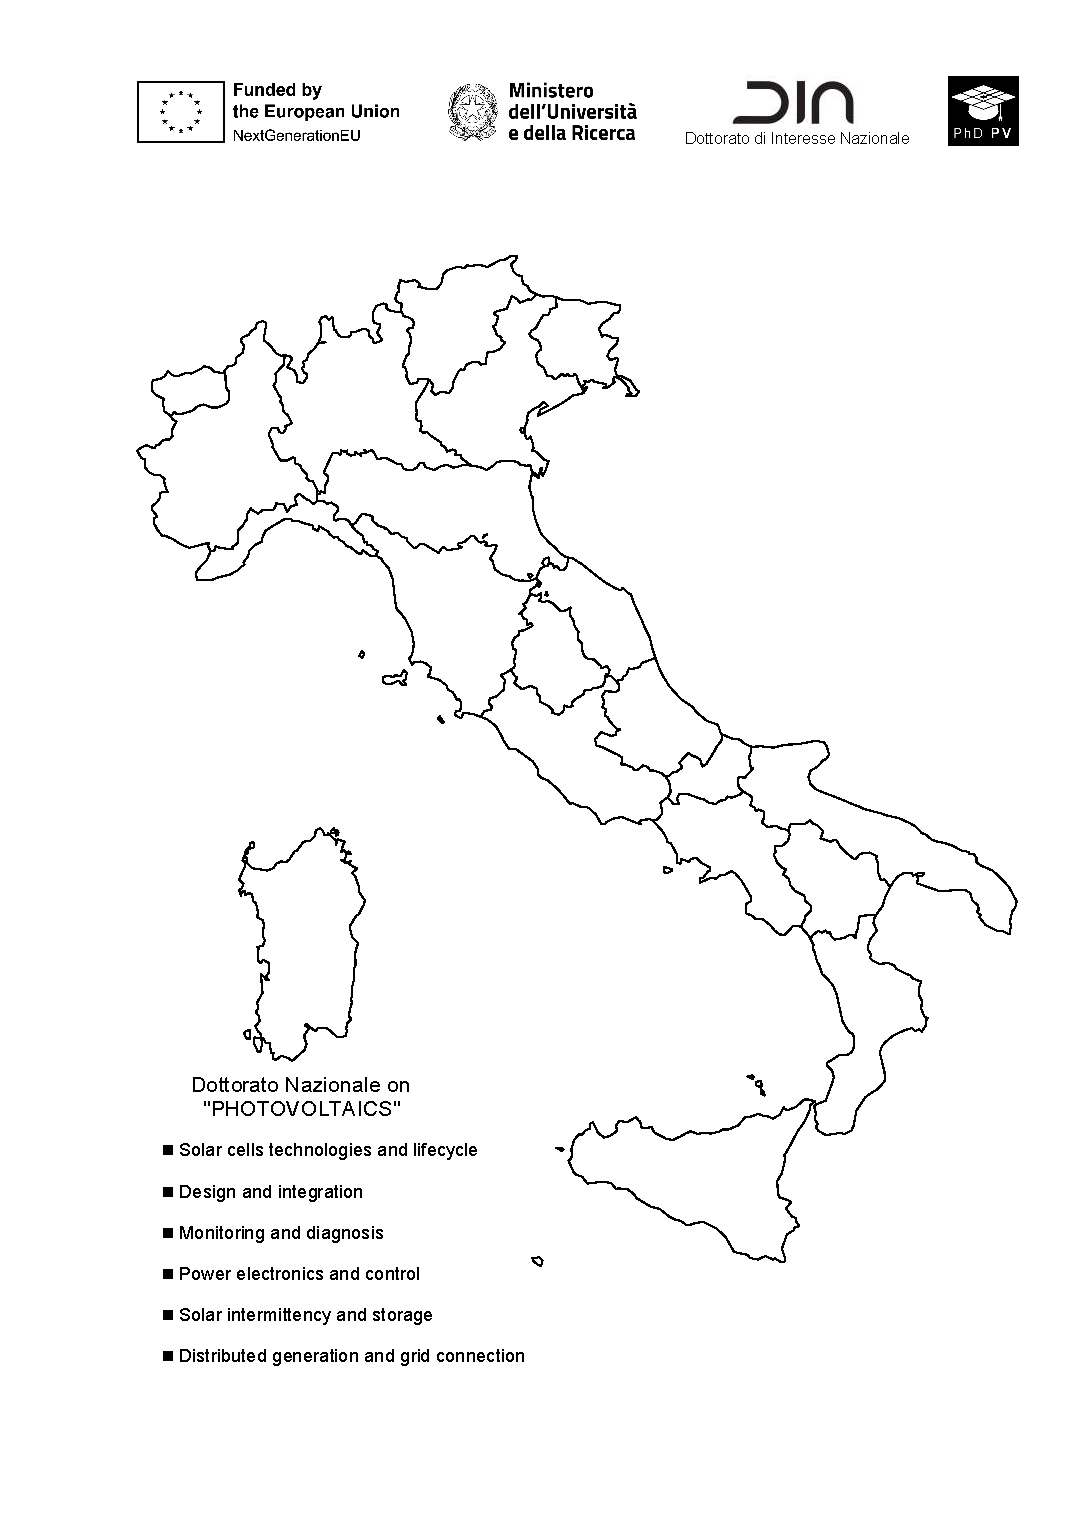
\includepdf[pages=1]{Figures/cover_page.pdf}
\cleardoublepage

% Dedication
\cleardoublepage
\begin{dedication}

    Dedicated to ...
    
\end{dedication}

% Table of Contents
\cleardoublepage
\tableofcontents
\clearpage
\sloppy
\hyphenpenalty=10000
\exhyphenpenalty=10000

% Lists of Figures and Tables
\clearpage
\listoffigures
\addcontentsline{toc}{chapter}{List of Figures}

\clearpage
\listoftables
\addcontentsline{toc}{chapter}{List of Tables}

% Inclusion of Chapters
\cleardoublepage        % Ensures the next page starts on an odd-numbered
\pagenumbering{arabic}  % Start numbering from this page
\setcounter{page}{1}    % Set this page as page 1
\pagestyle{headings}    % Apply regular page style for chapters

\chapter*{Abstract}
\blindtext[2] % Generates Lorem Ipsum

\chapter{Introduction}

Lorem ipsum dolor sit amet, consectetur adipiscing elit. Vivamus risus velit, malesuada non semper in, posuere in ante. Sed non luctus lacus. Curabitur sit amet ex dapibus, rhoncus nulla non, luctus leo. Fusce suscipit dolor quis erat dictum luctus. Nullam eget vulputate elit. Nam tristique, augue sit amet eleifend aliquet, felis mi egestas sapien, at tempus risus dui quis justo. Curabitur dictum nisl sit amet aliquam mollis. Cras hendrerit viverra neque, eu placerat nulla gravida ac. Sed sit amet massa euismod, pharetra ipsum sed, bibendum mauris. Etiam tempus vehicula leo sit amet tristique. Nulla sit amet tempus velit, sed pretium lectus. Cras sed nibh ut elit gravida dapibus at nec dui. Nunc et dolor at purus auctor aliquet sit amet imperdiet mi. Lorem ipsum dolor sit amet, consectetur adipiscing elit. In hac habitasse platea dictumst.

\section{Research Problem}

Fusce ut felis nec lacus faucibus aliquet at nec est. Nulla eleifend felis vitae velit blandit, et mattis lacus pretium. Aenean auctor semper ligula nec ornare. Aliquam varius, justo eu fringilla commodo, nunc est ullamcorper dolor, vel tristique sapien ante vel nulla. Duis feugiat rutrum aliquam. Pellentesque facilisis metus ac laoreet consectetur. Fusce euismod nisi a enim tristique, sit amet ullamcorper justo elementum. Morbi luctus posuere varius. Sed id rhoncus nisi. Duis non tellus nec ante maximus dignissim id non ante. Suspendisse et porta nisl, non pellentesque lacus. Mauris porttitor lorem id consectetur scelerisque. Nunc sit amet dolor sit amet erat cursus luctus pretium quis mauris.

Aliquam a nunc semper, ullamcorper est eu, ultricies mi. Ut interdum, diam sit amet vehicula ultrices, turpis massa ornare massa, et efficitur nulla tortor vitae lacus. Suspendisse facilisis ante et ex dignissim, sit amet rhoncus nunc sagittis. Morbi placerat neque eu justo sodales mollis. Sed ultricies aliquet mi et scelerisque. Donec volutpat malesuada felis sit amet luctus. Vivamus accumsan justo diam, blandit sodales odio rhoncus id. Suspendisse potenti. Sed et velit tristique, scelerisque enim at, posuere odio. Integer consectetur ante erat, id sagittis magna pharetra ut. Mauris aliquam, ipsum ac aliquam sollicitudin, urna neque elementum urna, sit amet pharetra ex nisi quis lacus. Vivamus consequat convallis ipsum, non volutpat nibh consequat at. Etiam in eros porta, condimentum tellus in, maximus est.

\section{Objectives}

Nulla euismod diam ornare tortor fermentum pharetra sed at erat. Pellentesque malesuada placerat maximus. Integer pharetra imperdiet sapien, id elementum elit efficitur sed. Phasellus quis placerat ex, in ultricies magna. Vivamus efficitur facilisis sapien, eget consectetur justo lacinia id. Nam nisi libero, tristique id fringilla at, ornare ut lacus. Vestibulum iaculis metus dapibus sapien finibus venenatis. Aliquam sed laoreet tortor. Mauris lacus metus, blandit at tempus egestas, congue sed quam. Nulla pulvinar ipsum eget tellus venenatis, ut gravida mi gravida. Aliquam efficitur gravida lectus, a semper velit ornare non. Etiam efficitur pellentesque tellus at aliquet. Curabitur placerat ac ex id vehicula~\cite{Topic1_Author_Year}.

Vivamus faucibus, lectus a tempus condimentum, elit mi maximus purus, eu iaculis ipsum turpis sed nisl. Pellentesque blandit velit non semper ultricies. Sed elementum nunc vitae dapibus mollis. Suspendisse viverra eu lacus quis fermentum. Nulla aliquet, sapien vel egestas hendrerit, lorem felis sagittis ante, at blandit lorem massa ut diam. Cras viverra tincidunt ante vel eleifend. Mauris vitae auctor tortor. Donec consectetur, sem dignissim hendrerit finibus, magna nibh imperdiet orci, sed volutpat dui tellus sit amet ligula. Suspendisse urna urna, tempor at tortor ac, dapibus volutpat metus. Sed a lacus ullamcorper, gravida justo sit amet, semper velit. Duis sodales viverra nisl, ut ultrices urna tristique eget. Duis imperdiet, mauris eu vestibulum lobortis, purus enim ultrices urna, eu ornare ante sapien sed nisi. Sed mollis placerat orci et posuere. Nunc egestas tortor iaculis, porta eros eget, mollis lorem~\cite{Topic2_Author_Year}.

\section{Thesis Structure}

Donec mattis tellus posuere, placerat ante quis, suscipit mauris. Ut fringilla ex diam, eget lobortis nisi ultricies vel. Pellentesque nulla leo, semper in accumsan in, interdum sit amet nulla. Aenean et bibendum mauris. Mauris placerat sit amet sapien id blandit. Nunc nulla nulla, fermentum sed auctor eget, consectetur vitae neque. Aenean et urna neque.

In et congue libero, eu aliquam arcu. Etiam eleifend est non enim volutpat rutrum ornare eget ante. Pellentesque dignissim suscipit augue, ut vulputate lacus volutpat quis. In volutpat sapien eget dignissim condimentum. Mauris sed suscipit libero, vel ornare dolor. Duis est eros, mattis eu diam malesuada, elementum ultrices eros. Nullam id viverra sem. Mauris quis erat quis odio tristique lobortis. Maecenas euismod quis purus in cursus. Sed posuere velit quis sapien consequat commodo. Maecenas volutpat pulvinar consectetur. Suspendisse quis urna sit amet est bibendum iaculis. Nam luctus tincidunt nulla, ut semper erat pretium eu.
\chapter{Literature Review}

Lorem ipsum dolor sit amet consectetur adipiscing elit. Quisque faucibus ex sapien vitae pellentesque sem placerat. In id cursus mi pretium tellus duis convallis. Tempus leo eu aenean sed diam urna tempor. Pulvinar vivamus fringilla lacus nec metus bibendum egestas. Iaculis massa nisl malesuada lacinia integer nunc posuere \gls{sdm}. Ut hendrerit semper vel class aptent taciti sociosqu. Ad litora torquent per conubia nostra inceptos himenaeos.~\cite{Topic2_Author_Year}. Lorem ipsum dolor sit amet consectetur adipiscing elit. Quisque faucibus ex sapien vitae pellentesque sem placerat. In id cursus mi pretium tellus duis convallis. Tempus leo eu aenean sed diam urna tempor. Pulvinar vivamus fringilla \gls{sdm} lacus nec metus bibendum egestas. Iaculis massa nisl malesuada lacinia integer nunc posuere. Ut hendrerit semper vel class aptent taciti sociosqu. Ad litora torquent per conubia nostra inceptos himenaeos~\cite{Topic1_Author_Year}. 

\section{Pulvinar vivamus fringilla}

Lorem ipsum dolor sit amet consectetur adipiscing elit. Quisque faucibus ex sapien vitae pellentesque sem placerat. In id cursus mi pretium tellus duis convallis. Tempus leo eu aenean sed diam urna tempor. Pulvinar vivamus fringilla lacus nec metus bibendum egestas. Iaculis massa nisl malesuada lacinia integer nunc posuere \gls{sdm}. Ut hendrerit semper vel class aptent taciti sociosqu. Ad litora torquent per conubia nostra inceptos himenaeos.

\section{Iaculis massa nisl malesuada}

Suspendisse et viverra felis. Integer eu venenatis risus. Etiam et porttitor turpis. Nam hendrerit commodo dui et malesuada. Quisque cursus, libero vel mattis tincidunt, tortor libero aliquet ligula, id euismod quam est nec nibh. Maecenas semper est nibh, sed molestie metus interdum at. Duis faucibus, sem a sodales mollis, sem elit eleifend purus, in egestas orci magna vitae erat. Sed tristique massa mi, id auctor metus elementum sed. Aliquam malesuada ex neque, consectetur vehicula arcu vulputate sed. Vestibulum faucibus dolor urna, ac volutpat lectus volutpat non. Vestibulum id neque pharetra, luctus erat in, tincidunt nisi.

Integer ut faucibus urna, eget convallis felis. Etiam facilisis molestie tellus et lacinia. Ut urna mauris, malesuada vel est et, pulvinar facilisis lorem. Ut eu lectus nulla. Ut sit amet orci at lorem ultricies ullamcorper. Proin odio justo, ultrices id lorem non, suscipit tempus odio. Nulla interdum nisi et eleifend placerat. Fusce rutrum nibh ut posuere eleifend. Vestibulum sodales eros ut libero ornare, non varius urna mollis. Donec sed porttitor nunc. Integer euismod nunc ex, id facilisis lectus tincidunt ut. Curabitur gravida, arcu sit amet gravida tincidunt, metus est dapibus magna, ut iaculis neque magna ut nibh. Nulla gravida lectus nec tellus congue, sit amet dictum metus laoreet. Fusce a tincidunt ipsum, vitae placerat est \gls{sdm} lacus nec metus bibendum egestas. Iaculis massa nisl malesuada lacinia integer nunc posuere. Ut hendrerit semper vel class aptent taciti sociosqu. Ad litora torquent per conubia nostra inceptos himenaeos~\figref{fig:placeholder_example}.

    \begin{figure}[hbtp!]
        \centering
        
\includegraphics[width=0.5\linewidth]{Figures/image.png}
        \caption{Example caption for a figure.\\ \textit{Additional explanations can be added}}
        \label{fig:placeholder_example}
    \end{figure}

Phasellus posuere consequat lectus eu fringilla. In interdum fermentum quam in tempus. Cras at ligula urna. Donec non lorem elit. Etiam rhoncus nec neque quis mollis. Class aptent taciti sociosqu ad litora torquent per conubia nostra, per inceptos himenaeos. Etiam ac nisl dolor. Aenean eu justo magna. Fusce tristique nisl aliquet tempor rutrum. Curabitur nec semper sapien. Suspendisse maximus dapibus nunc ac efficitur. Aenean mollis ornare urna eu hendrerit. Suspendisse eu lorem egestas, laoreet orci eget, finibus ligula. Vestibulum vel dictum diam. Vivamus at magna dui. Sed fermentum, sapien id imperdiet iaculis, augue lacus tempus ex, vitae pulvinar arcu ligula quis lectus. Nulla odio diam, fringilla sed sapien vitae, porta venenatis dui. Integer varius ac erat eu bibendum. Nam sed mollis ligula, in finibus magna. Nunc id pretium libero, eget bibendum diam. Vivamus laoreet nec nulla ultricies varius. Aliquam id molestie nisl. Nunc vehicula convallis libero, a pretium ante vehicula sit amet. Nunc consequat tortor vitae dignissim cursus.

Phasellus eget gravida ligula. Interdum et malesuada fames ac ante ipsum primis in faucibus. Vivamus tempus cursus magna id aliquet. Vivamus vel gravida lectus, tempus porttitor massa. Aenean condimentum ex purus, nec fringilla nibh suscipit vel. Sed tempor dolor ac felis molestie, eget consectetur dolor tristique. Sed non eros pulvinar, porttitor purus in, viverra nunc. Vestibulum eleifend turpis felis, eu ullamcorper lectus pulvinar sit amet. Donec sagittis sapien leo, ac laoreet eros tincidunt non. Donec nulla arcu, imperdiet eget rhoncus in, congue ac quam. Fusce tristique nec nisl at fermentum. Vestibulum congue, odio placerat iaculis facilisis, tortor dui pulvinar est, in elementum tortor tortor a est. Nulla eu orci tortor. Suspendisse commodo et magna vitae venenatis. Ad litora torquent per \gls{sdm} conubia nostra inceptos himenaeos~\tabref{tab:placeholder_table}.

    \begin{table}[ht]
    \centering
        \begin{tabular}{|l|l|l|l|l|}
            \hline
            \textbf{Parameter} & \textbf{Unit} & \textbf{Test 1} & \textbf{Test 2} & \textbf{Test 3} \\ \hline
            Input Voltage      & V             & 12.0            & 11.8            & 12.2            \\ \hline
            Output Current     & A             & 1.5             & 1.6             & 1.4             \\ \hline
            Efficiency         & \%            & 92.3            & 91.8            & 93.1            \\ \hline
            Temperature Rise   & °C            & 32              & 34              & 31              \\ \hline
        \end{tabular}
        \caption{Performance comparison of the table caption.}
        \label{tab:placeholder_table}
    \end{table}

\section{Sed fermentum}

Aliquam dui justo, eleifend non tempus quis, fringilla nec ante. Fusce varius nulla sit amet erat dapibus gravida. Nam vitae turpis nunc. Nulla convallis ultricies dolor, id luctus mi rhoncus vel. Vivamus pharetra laoreet massa eget aliquet. Donec in diam in ligula accumsan aliquet. Morbi fringilla non massa eget pulvinar. Aenean sit amet posuere felis, sed iaculis tortor. Sed cursus, nibh sed ullamcorper finibus, purus libero malesuada leo, et porta purus orci a nisi. Nam sit amet justo tortor. Donec ac ex aliquam orci facilisis porttitor. Morbi finibus, nibh at mattis sollicitudin, nunc nunc lobortis justo, sed vehicula neque urna a odio \equref{eq:placeholder_equation}.

    \begin{equation}
        i_{pv}(t) = i_{ph}(t) - i_{D}(t) - i_{R_{sh}}(t)
        \label{eq:placeholder_equation}
    \end{equation}

Nam sed odio nulla. Cras et velit in ex tempus cursus. Etiam scelerisque sapien at pulvinar placerat. Cras consequat nunc ligula, sit amet facilisis mauris fringilla vel. Sed blandit porttitor elit non laoreet. Duis placerat purus eget magna varius suscipit. Aliquam est tortor, tincidunt vitae odio ut, egestas convallis sapien. Donec ex turpis, eleifend at est nec, dictum egestas neque. Maecenas mollis tortor mauris, ut mattis purus volutpat sed. Vestibulum erat velit, auctor vitae felis et, tempor rhoncus sem. Etiam ut metus ante. Sed in tortor tincidunt, fermentum risus vitae, ultricies nibh. Vivamus libero ante, mollis quis leo non, pulvinar efficitur odio. Duis tincidunt dolor at nisl viverra posuere. Nullam finibus scelerisque velit, vel volutpat dolor auctor quis.

% \chapter{Introduction}
% \blindtext[7] % Generates Lorem Ipsum

% \chapter{Literature Review}
% \blindtext[7] % Generates Lorem Ipsum

\chapter{Methodology}
\blindtext[5] % Generates Lorem Ipsum

\chapter{Results and Discussion}
\blindtext[7] % Generates Lorem Ipsum

\chapter{Conclusion}
\blindtext[3] % Generates Lorem Ipsum

% Acknowledgements
\chapter*{Acknowledgements}
\thispagestyle{empty}
\markboth{ACKNOWLEDGEMENTS}{}
\addcontentsline{toc}{chapter}{Acknowledgements}
\blindtext[1] % Generates Lorem Ipsum

% Bibliography
\clearpage
\bibliographystyle{ieeetr}
\bibliography{references.bib} % Make sure this file exists

\clearpage
\end{document}